\documentclass{article}
\usepackage{pdfpages}
\usepackage{hyperref}
\usepackage{parskip}
\usepackage[a4paper,margin=1in]{geometry}
\usepackage{soul}

\title{Solutions to the 1000 star maps}
\author{Cheng Ian and Kane}
\date{October 2024}

\usepackage{titling}
\renewcommand\maketitlehooka{\null\mbox{}\vfill}
\renewcommand\maketitlehookd{\vfill\null}

\pagenumbering{gobble}
\begin{document}

\begin{titlingpage}
\maketitle
\end{titlingpage}

\section{Introduction}
This document is our (Cheng Ian and Kane) attempt at doing 1000 star maps by hand. The star maps are sourced from \url{https://tinyurl.com/sidpro1000}, made by Sidharth a while back. In case this link goes dead, you can use \url{https://github.com/pgot/1000-star-maps/raw/main/1000%20star%20maps.pdf}; most of the resources for this document are on the same repository (\url{https://github.com/pgot/1000-star-maps}). If you want to generate these charts yourself, you can use \url{https://www.fourmilab.ch/cgi-bin/Yoursky}, setting the colour to black on white, and unchecking all the display options.

\section{How to read the charts}
\subsection{Before starting}
Before starting to mark out the charts, there's a couple of things to note. For the basics, each dot represents a star, with larger dots representing brighter stars, from magnitude 5.5 and below. Notably, \textit{planets are not shown.}

The circle is a stereographic projection of the sky at some random location, and exactly half the sky is shown. The cardinal points are also shown on the outer rim of the circle, and North-South \textit{always} runs up-down on the page.
\subsection{Markings}
There are several types of marks on the charts. These include constellation lines, constellation labels (some), equator/ecliptic/galactic great circles (some), Deep Sky Object (DSO) markings, and star designations.

Constellation lines are drawn as solid lines, and always stay within constellation boundaries (notably except \(\beta\) Tauri and \(\alpha\) Andromedae, but these stars were ambiguous in their naming and which constellation they'd belong). Some dim constellations (e.g. Mensa, Sextans, Camelopardalis) are not drawn with constellation lines sometimes, due to the stars involved being to dim to be notable. The constellation lines are not agreed upon absolutely, and can vary from source to source. These lines are based on the constellation lines in Stellarium. Some of these constellations may be labeled with their names or their 3-letter IAU abbreviations, especially for star maps closer to the beginning.

DSOs are marked by a cross at their locations, with their catalog number above them. If there are many notable DSOs at a particular location, these may be condensed with the use of commas, giving up some accuracy of location for readability. We note down DSOs from the Messier Catalog and notable objects from the Caldwell catalog (for some). Objects from the Messier catalog are listed as their catalog number without prefix, while Caldwell catalog objects are listed with the prefix "C". When condensing objects from different catalogs, Messier objects are listed first, followed by the prefix "C" and the Caldwell catalog numbers (e.g. 103, C8, 10, 13 means Messier 103, Caldwell 8, Caldwell 10, Caldwell 13). Some notable New General Catalog objects are noted with NGC, although we don't note virtually all of them (except \#813).

Star designations are noted with their catalog number/Bayer designation written next to the star without any crosses/marks. Bayer designations are (as usual) Greek letters, and numbers without prefix are Flamsteed designations. Stars noted that do not fall into these catalogs are noted with their well-known catalog abbreviations (e.g. HIP, HD).
\section{Final notes}
This attempt used 500 sheets of paper, with work done from March 2022 to August 2024. We recommend doing less than 1000, and preferably digitally, so that paper is not wasted in large amounts like in our case.

Importantly, \ul{\textbf{not everything important may be marked, and not everything marked is correct}}.This was a hobby project both of us did in our free time, which stemmed from planning to revise after the Singapore Astronomy Olympiad was over. Most of this free time was from being bored and sleepy in class, leaving up the potential for errors to appear and persist through multiple star maps. Some arguably important objects, constellations and stars may not be labeled as well. We apologize for the lack of completeness.

Also, some of these papers were used for other purposes (such as scratch paper for homework), and may have lots of other stuff written on them. This includes the derivation of the Friedmann equations through general relativity, nim-values for the impartial knight (and other derivations from combinatorial game theory), the Heart Sutra and rock-paper-scissors-101 among other things. Some of the drawings below the star maps, e.g. on \#1000, are from our friend Greene, although the markings on the star maps are mostly from us.

These star maps have also traveled with us to Switzerland, Poland and Brazil, and some contestants in the 2023 IOAA have done some small parts of these. One of the star maps has been taken to Saudi Arabia by one of their contestants who was keen to try one.

We would like to thank everyone who made this possible, from Sidharth making the original document, NUS High for providing a ream of paper and mass printing and scanning capabilities, all the people we've met at IOAA, and everyone else who was at least tolerant of us doing this.
\includepdf[pages=-]{1 to 1000 filled edit.pdf}
\newpage
\vspace*{\fill}
\begingroup
\centering
\textbf{Addendum}

The following star maps are included due to printing errors and miscommunication. They are duplicates of the star maps featured above.

\endgroup
\vspace*{\fill}
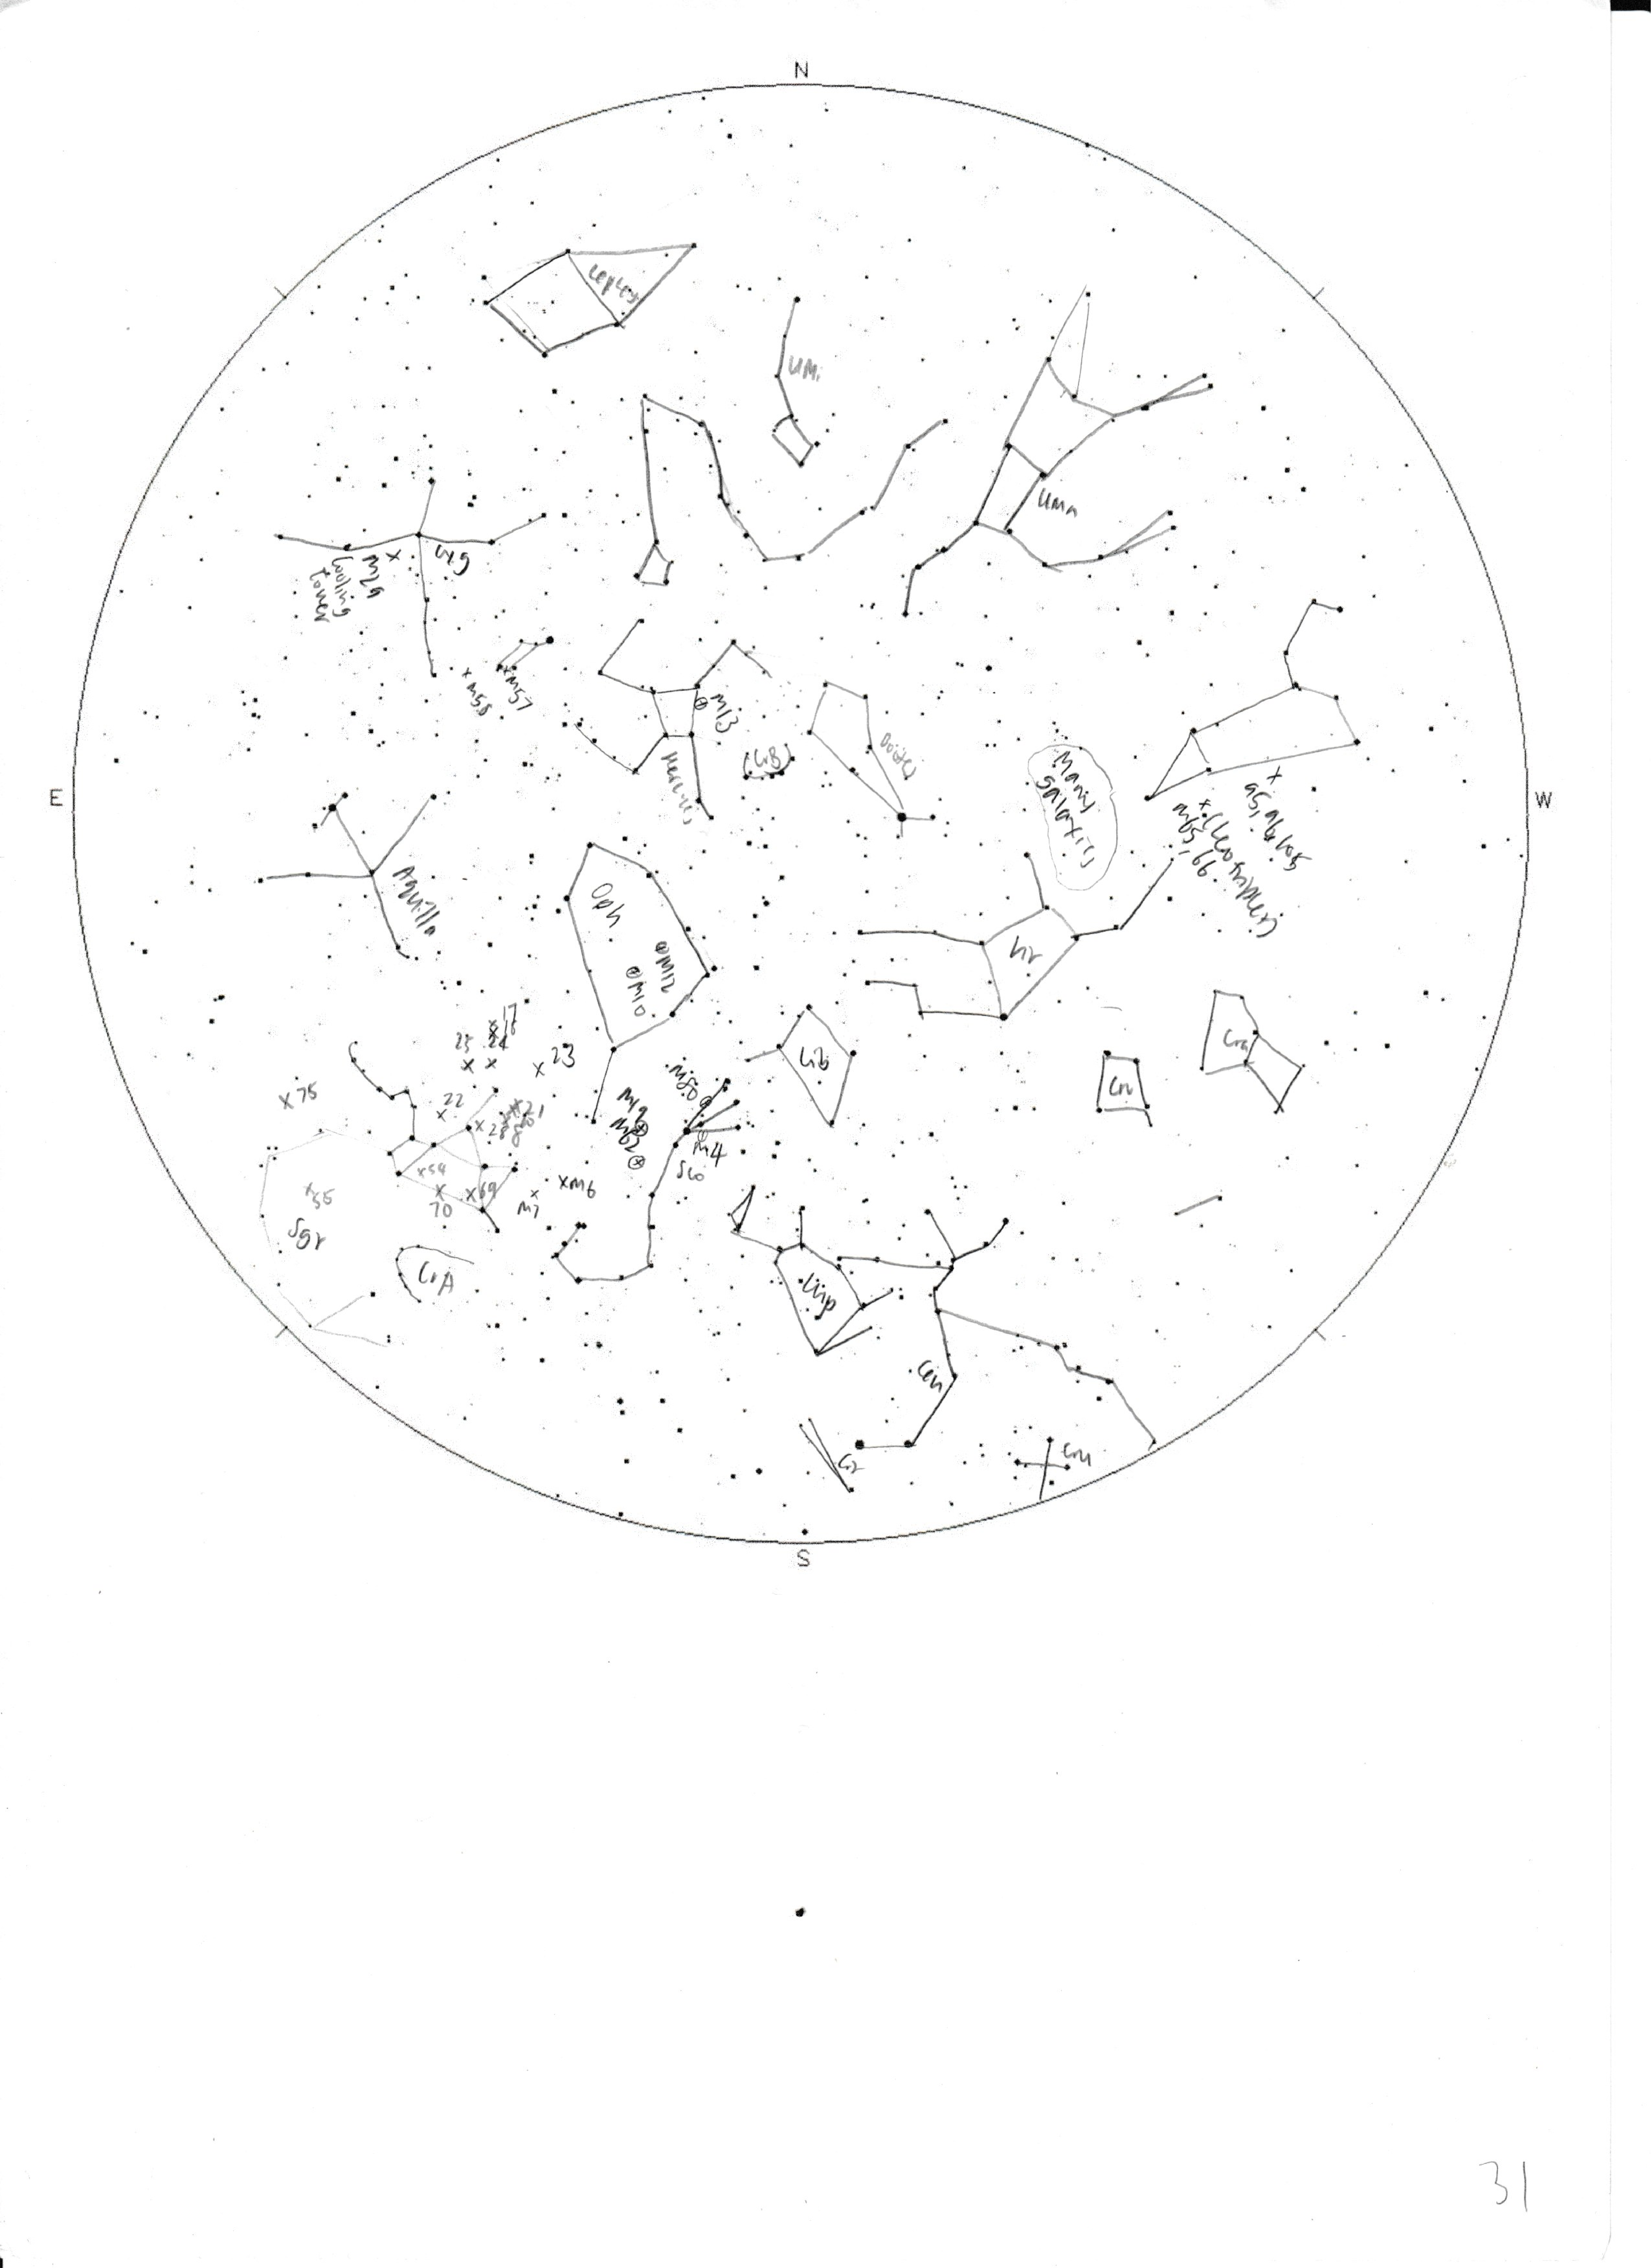
\includepdf[pages=-]{addendum/31.pdf}
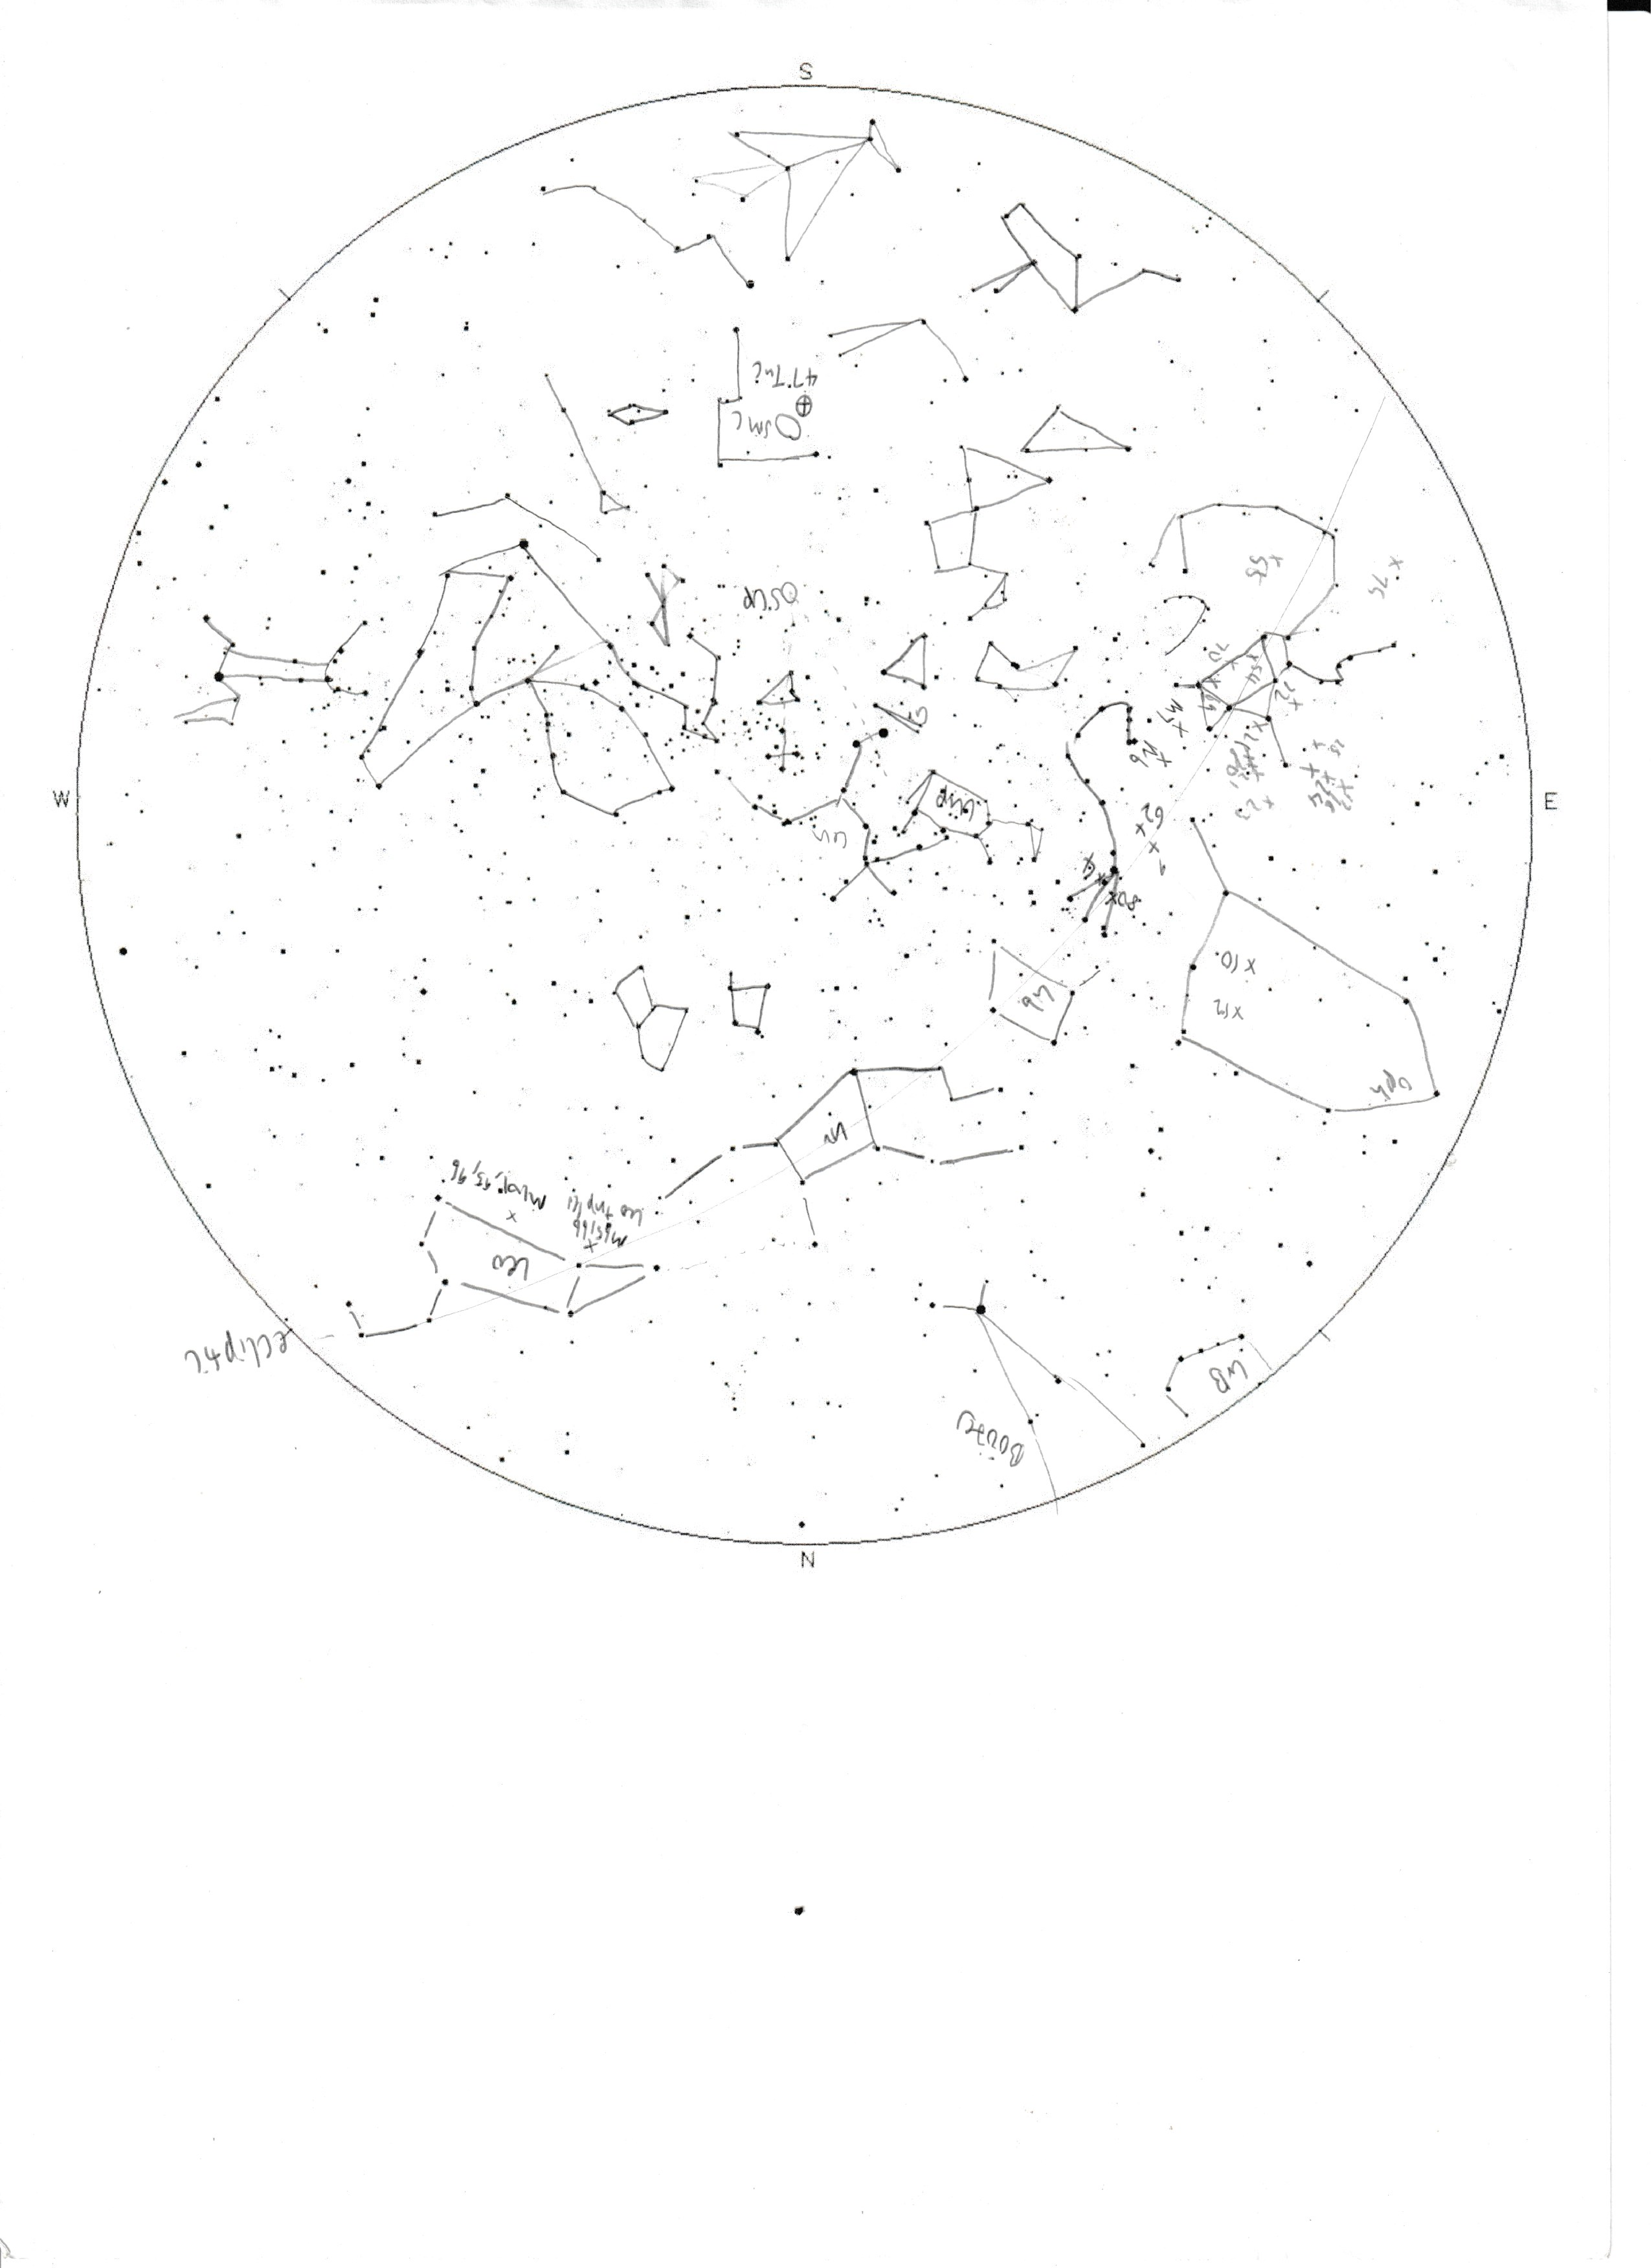
\includepdf[pages=-]{addendum/32.pdf}
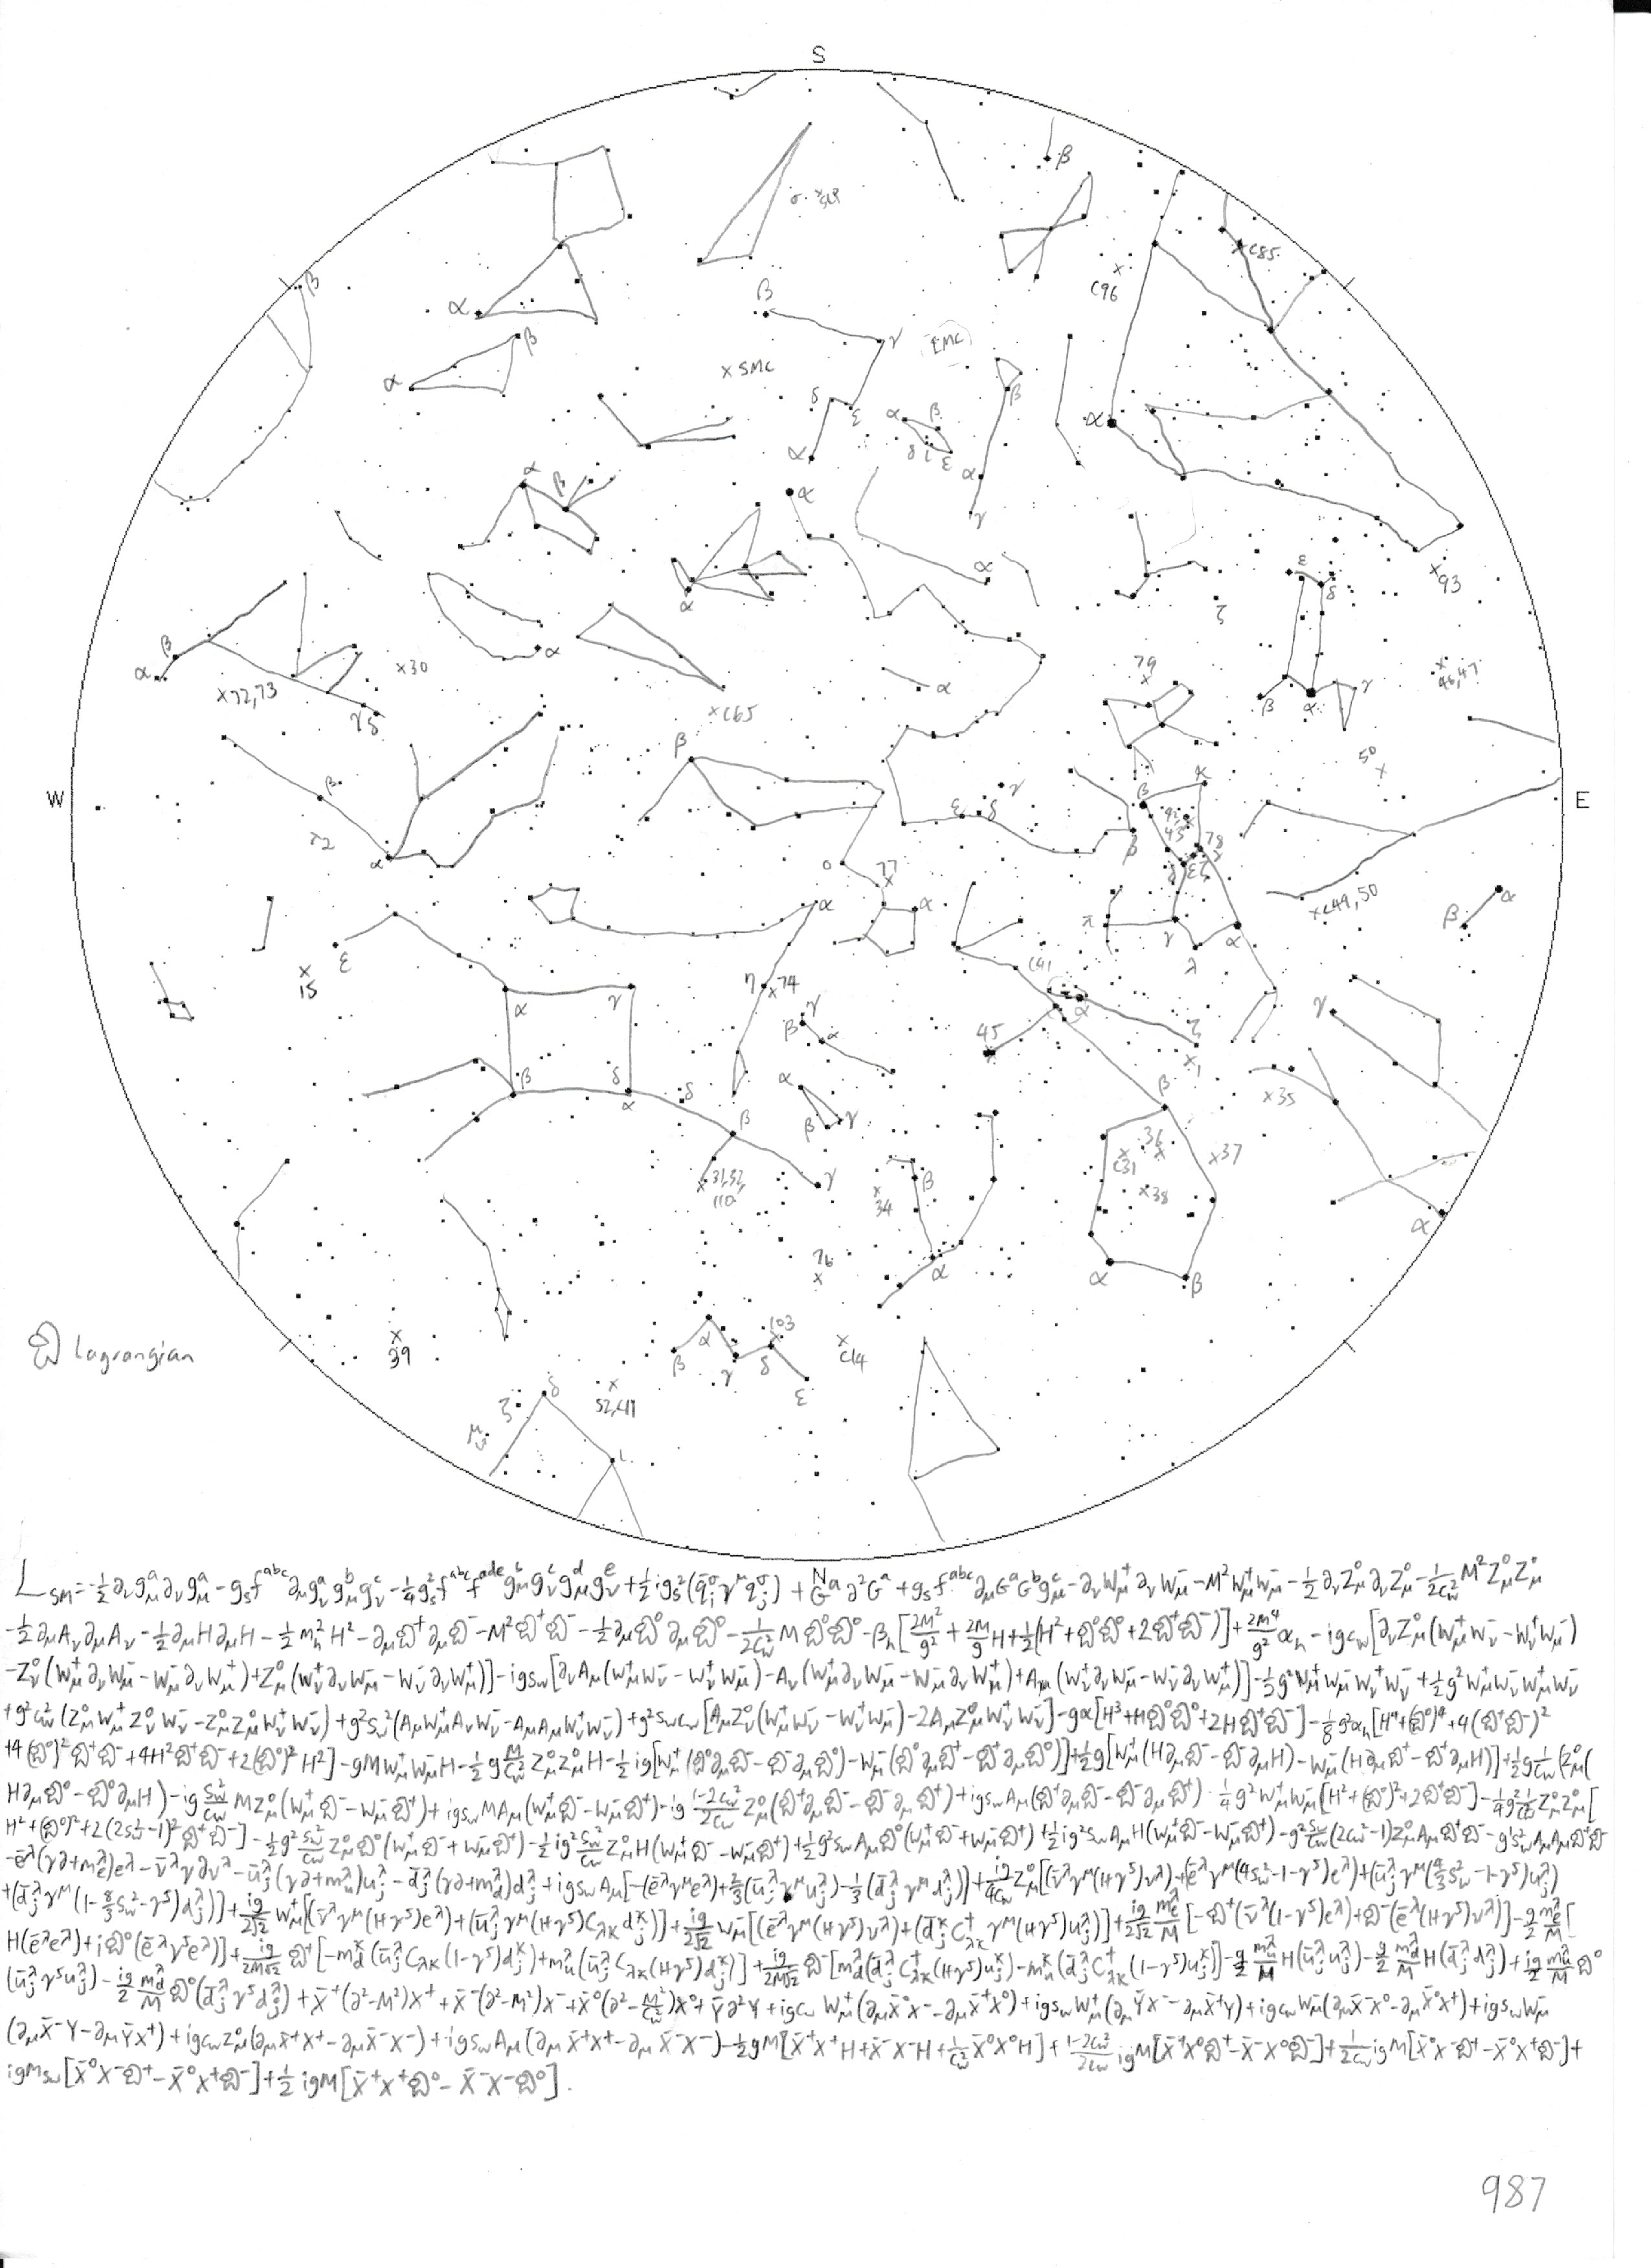
\includepdf[pages=-]{addendum/987.pdf}
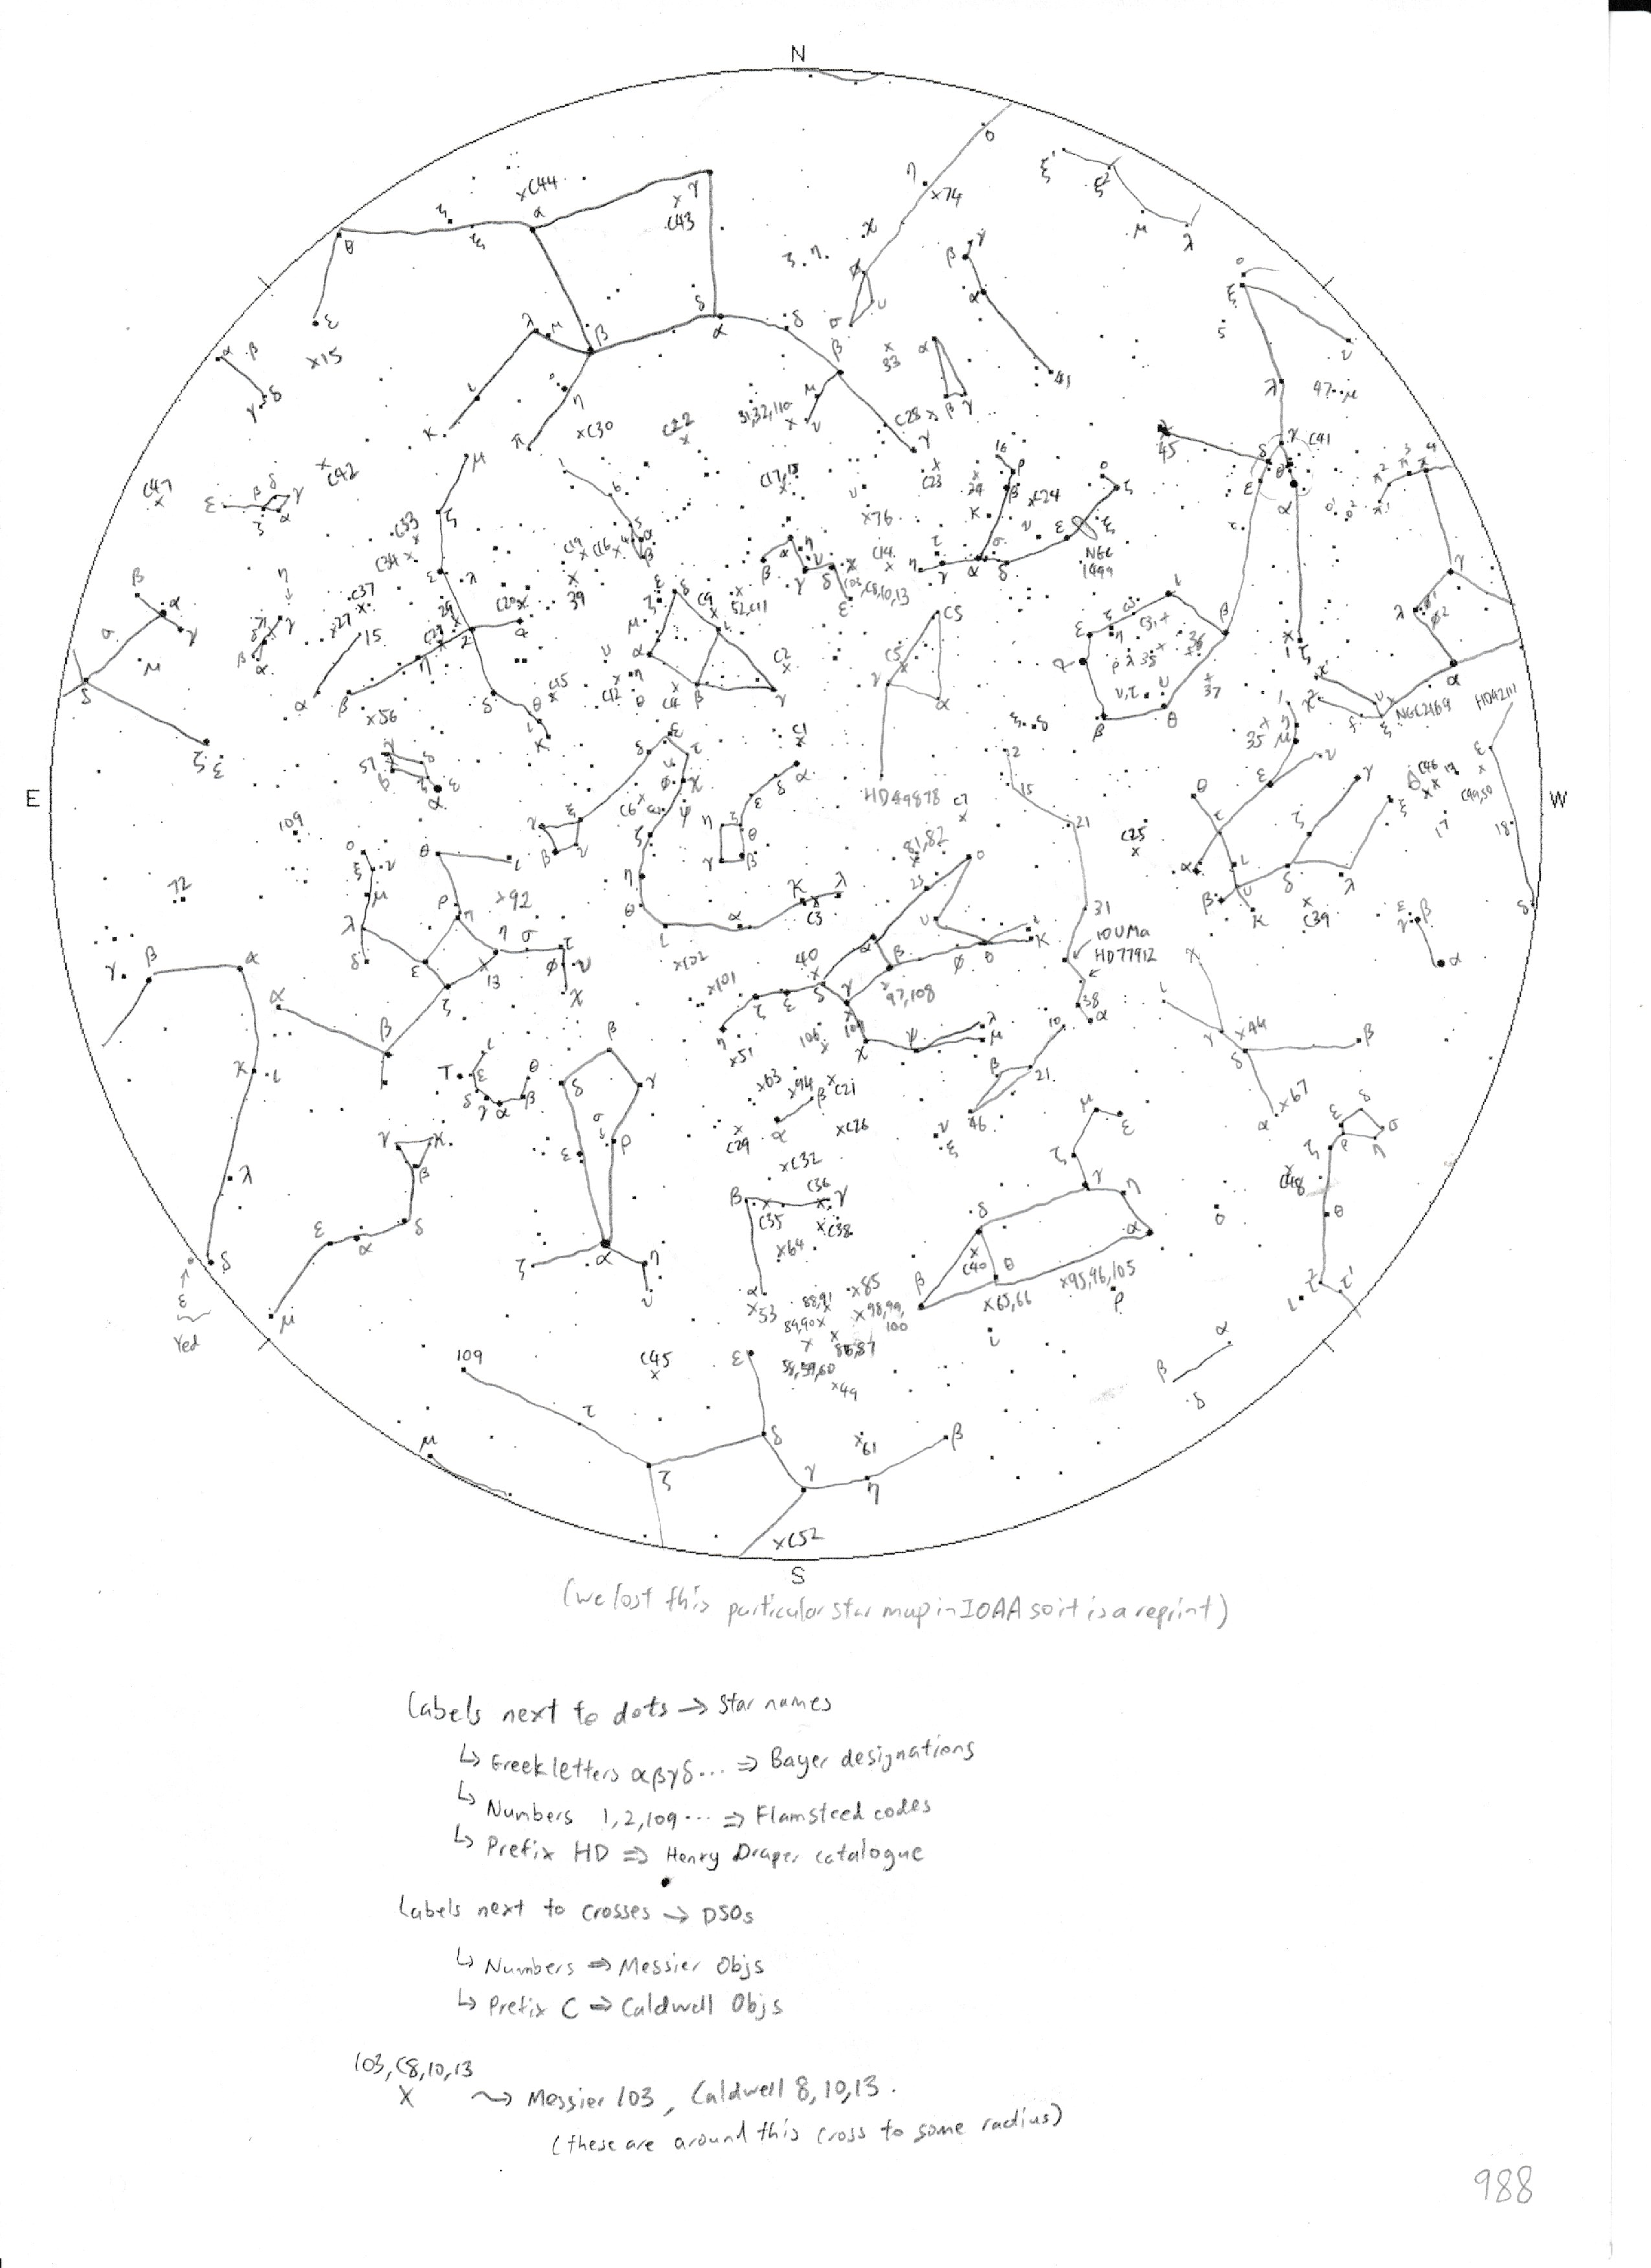
\includepdf[pages=-]{addendum/988.pdf}
\end{document}
